\chapter{Implementation}
\label{cha:implementation}

\section{Work plan --- Work packages, deliverables}
\label{sec:work-plan}

\subsection{Overall structure}
\label{sec:wpstructure}

The overall approach to the work plan is to have the research and development of the selection function progress in parallel with the implementation thereof. We made this choice because of the complexities of the selection function and its realization in the form of tools and auxiliary data, and because of the relatively short duration of the project. The work flow we foresee for {\acro} is shown in \figref{fig:workflow}. It is an iterative workflow in which the findings in each of work packages \ref{wp:selfungaia}--\ref{wp:scienceappl} will inform the others. For example the research on the selection function will lead to requirements on the implementation, while at the same time the conversion of research ideas into practical tools will lead to the questioning and revision of those same ideas.

At several points during the project the results will be combined into prototype implementations of the selection function tools. These will be tested both internally to the project and through the public availability of one prototype implementation. Specifically, we plan to organize two community workshops just after the public release of the prototypes to train members from the astronomical community in the use of the tools and to collect user feedback. The results from these tests will feed into the next round of research, development, and implementation. The scientific nature of much of the work conducted in {\acro} will very much benefit from an iterative approach. Close coordination between the work packages will of course be essential and this is foreseen in the management structure.

\begin{figure}
    \centering
    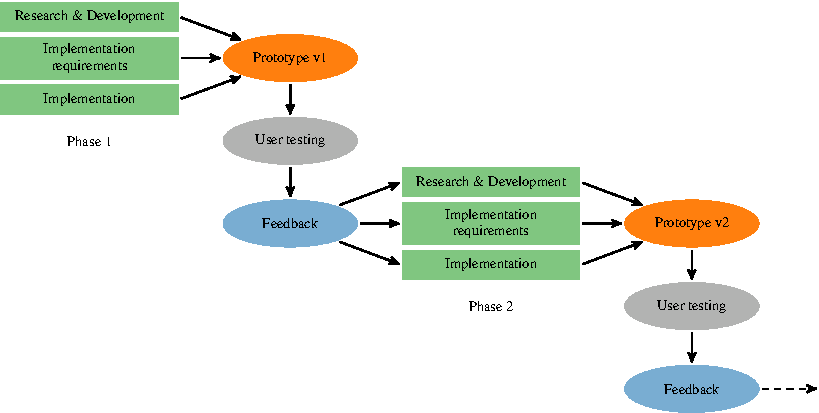
\includegraphics[width=\linewidth]{workflow.pdf}
    \caption{Iterative workflow for {\acro}.}
    \label{fig:workflow}
\end{figure}

\begin{figure}[ht!]
    \centering
    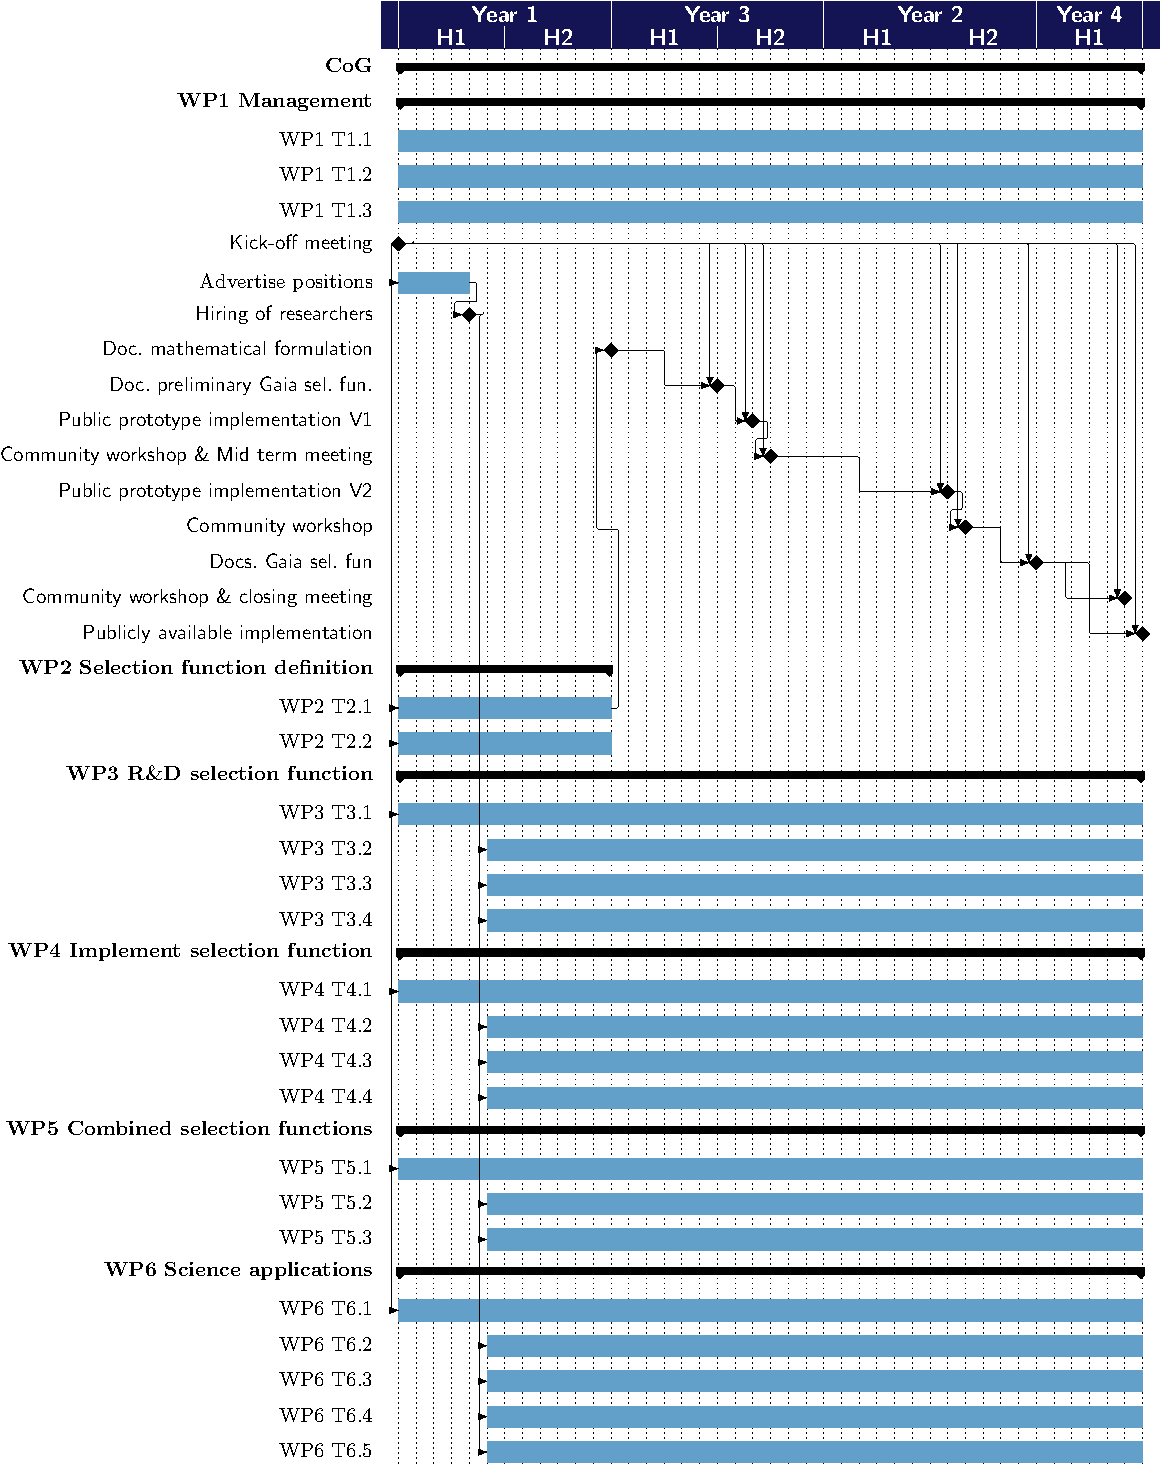
\includegraphics[width=\linewidth]{cog-gantt.pdf}
    \caption{Gantt chart for the {\acro} project.}
    \label{fig:gantt}
\end{figure}

\subsection{Timing of the work packages}
\label{sec:wptiming}

The overall work plan is structured as follows:
\begin{itemize}
    \item The first 6 months will be used to recruit the researchers to be funded from this proposal and to carry out the tasks in work package \ref{wp:selfundefinition}. Having a mathematical framework for the selection function in place early on in the project is important for guiding the research and the implementation phases.
    \item During the next three years of the project the efforts in work packages \ref{wp:selfungaia} to \ref{wp:scienceappl} will happen mostly in parallel for the reasons outlined above. The iterative approach outline in \secref{sec:wpstructure} will be used in this phase.
    \item The selection function implementation prototypes to be developed in each phase will increase in their level of detail and complexity. Initially we may chose to implement a prototype selection function that depends only on sky position and apparent magnitudes (\figref{fig:gsf_ideal}), without any consideration for observation interruptions on the spacecraft, or on-board or ground processing effects. For the second prototype it is natural to include spacecraft outages, as these events are well-documented. Depending on the level of complexity envisaged, Prototype 3 may include on board processing effects like magnitude estimates (given the input source catalogue) and telemetry effects. Later prototypes could include pipeline data processing interventions that occur on the ground, or how astrophysical environments would affect the observable properties (e.g., binarity, variability). The scope of each prototype will be iteratively guided by user testing, feedback, and the executive board. We explicitly foresee two public prototypes (see \figref{fig:gantt} and \secref{wp:selfunimplementation}, which will be presented and tested at two community workshop. Further internal prototypes are also foreseen.
 \end{itemize}

\makewplist

%\subsection{Work package description}
%\label{sec:wps}

\tablecaption{Description of work packages}
\begin{supertabular}{p{\textwidth}}
    \omit \tabularnewline
\end{supertabular}
%%%%%%%%%%%%%%%%%%%%%%%%%%%%%%
%  Work Package Description  %
%%%%%%%%%%%%%%%%%%%%%%%%%%%%%%

\begin{workpackage}{Management}
  \label{wp:management} %change and use appropriate description

  %%%%%%%%%%%%%%%%%% TOP TABLE %%%%%%%%%%%%%%%%%%%%%%%%%%%%%
  % Data for the top table
  \wpstart{1} %Starting Month
  \wpend{\duration} %End Month
  \wptype{MGT} %RTD, DEM, MGT, or OTHER
  \wplead{ULEI}

  % Person Months per participant (required, max 7, * for leader)  
  % syntax: \personmonths{Participant number}{value}    (not wp leader)
  %     or  \personmonths{Participant short name}{value} (not wp leader)
  %         \personmonths*{Participant number}{value}    (wp leader)
  % for example:
  \personmonths*{ULEI}{8}
  \personmonths{MPIA}{2}
  \personmonths{INAF}{2}
  \personmonths{UCAM}{2}
  \personmonths{NYU}{1}
  \personmonths{MONA}{1}
  % etc.

  \makewptable % Work package summary table

  % Work Package Objectives
  \begin{wpobjectives}
    This package provides the overall scientific coordination and administrative management of \acro\ as described in \secref{sec:management}.
  \end{wpobjectives}

  % Work Package Description
  \begin{wpdescription}
    % Divide work package into multiple tasks.
    % Use \wptask command
    % syntax: \wptask{leader}{contributors}{start-m}{end-m}{title}{description}   

    This work package includes the administrative tasks to fulfil the EC requirements and rules as well as the global administrative and coordination tasks inside the consortium, including financial management, intellectual property management, project documentation, and communication and dissemination activities. It also includes the coordination with institutions and bodies relevant for the development of the Gaia archive like ESA, DPAC and MW-Gaia, as well as the representation of {\acro} in meetings or committees related to this coordination.

    \wptask{ULEI}{ULEI}{1}{\duration}{Overall coordination}{
      \label{task:wp1coordinator}
      Overall coordination and administrative management as described above (6 ULEI person-months). The coordinator will be aided in his tasks by the Leiden Observatory project support staff.
    }
    \wptask{ULEI}{MPIA, INAF, UCAM, MONA, NYU}{1}{\duration}{Scientific coordination}{
      \label{task:wp1others}
      Scientific coordination by the four main partners through the {\acro} Executive Board (2 person-months each for MPIA/INAF/UCAM, 1 person-month each MONA/NYU). As stated in \secref{sec:management}, the partners NYU and MONA will have a standing invitation to meetings of the Executive Board in order to keep communications efficient.
    }
    \wptask{ULEI}{All other}{1}{\duration}{Communications and dissemination}{
      \label{task:wp1comms}
      Ensure that results from {\acro} are disseminated to the astronomical community through the appropriate academic channels (publications, conference presentations, community workshops, 2 ULEI person-months). Engage the astronomical community by making available prototype implementations of the tools developed as part of {\acro} and provide channels for feedback. Organize three community workshops to provide training on the use of the selection function implementations and to collect feedback on the {\acro} tools.
    }
  \end{wpdescription}
  
  % Work Package Deliverable
  \begin{wpdeliverables}
    % Data for the deliverables and milestones  tables
    % syntax: \deliverable[delivery date]{nature}{dissemination
    % level}{description} 
    %
    % nature: R = Report, DEM = Demonstrator, DEC = Websites, media, etc, OTHER = Other
    % dissemination level: PU = Public, CO = Confidential, CI = CLassified.
    % 
    % \wpdeliverable[date]{R}{PU}{A report on \ldots}

    The deliverables of this work package are the periodic and final reports for the EC, the consortium agreement (\secref{sec:cons_agreement}), the data management plans, and the organisation of the {\acro} plenary meetings (\secref{sec:procedures}) and community workshops.

    \wpdeliverable[1]{ULEI}{OTHER}{PU}{Kick-off meeting (plenary)}\label{dev:wp1kickoff}
    \wpdeliverable[2]{ULEI}{R}{PU}{Consortium agreement}\label{dev:wp1consortium_agreement}
    \wpdeliverable[6]{ULEI}{R}{PU}{Data management plan}\label{dev:wp1datamanagement}
    \wpdeliverable[13]{ULEI}{R}{PU}{First year report to EC}\label{dev:wp1year1report}
    \wpdeliverable[21]{ULEI}{OTHER}{PU}{Community workshop and mid-term meeting (plenary)}\label{dev:wp1midtterm}
    \wpdeliverable[25]{ULEI}{R}{PU}{Second year report to EC}\label{dev:wp2year1report}
    \wpdeliverable[32]{ULEI}{OTHER}{PU}{Community workshop}\label{dev:wp1community}
    \wpdeliverable[41]{ULEI}{OTHER}{PU}{Community workshop and closing meeting (plenary)}\label{dev:wp1closing}
    \wpdeliverable[\duration]{ULEI}{R}{PU}{Final report to the EC}\label{dev:wp1finalreport}
  \end{wpdeliverables}

\end{workpackage}


%%% Local Variables:
%%% mode: latex
%%% TeX-master: "proposal-main"
%%% End:

\begin{workpackage}{Definition of the selection function}
  \label{wp:selfundefinition}
  \wpstart{1} %Starting Month
  \wpend{12} %End Month
  \wptype{RTD} %RTD, DEM, MGT, or OTHER
  \wplead{MPG}
  \personmonths{ULEI}{1}
  \personmonths*{MPIA}{2}
  \personmonths{INAF}{1}
  \personmonths{UCAM}{1}
  \personmonths{NYU}{1}
  \personmonths{MONA}{1}
  
  \makewptable % Work package summary table

  % Work Package Objectives
  \begin{wpobjectives}
    This objective of this work package is to research and implement a precise mathematical formulation of the concept of a survey selection function. The results will be written up as a scientific paper (to be published in the peer-reviewed literature) that will guide the rest of the work to be done within {\acro}.  The mathematical formulation of the selection function will account for the following aspects:
    \begin{itemize}
        \item Applicability to arbitrary astronomical sky surveys.
        \item The combined selection function of multiple surveys can be described within the same formalism.
        \item Accommodate multiple selection layers (e.g., the selection function intrinsic to a survey combined with additional selections imposed by the user of the data).
        \item Unknowable aspects of the selection function should be accounted for (e.g., it is not guaranteed that all sources of data loss along the detection-telemetry-processing chain for Gaia can be traced). \memo{Formulate this more precisely and in a way that makes clear this aspect can be addressed.} \By{ARC}{Unknowable aspects of the selection function should be included. For example, it is not guaranteed that all sources of data loss along the detection-telemetry-processing chain for Gaia can be traced, but this can be approximated through knowing which repeated measurements were included in the catalog when expected.}
        \item ...
    \end{itemize}
  \end{wpobjectives}

  % Work Package Description
  \begin{wpdescription}
    % Divide work package into multiple tasks.
    % Use \wptask command
    % syntax: \wptask{leader}{contributors}{start-m}{end-m}{title}{description}   

    \wptask{MPIA}{MPIA}{1}{12}{Scientific coordination}{
      \label{task:wp2coordination}
      Scientific coordination of the work on defining the selection function and coordination of writing the paper corresponding to deliverable \ref{dev:wp2document}.
    }
    \wptask{MPIA}{All other}{1}{12}{R\&D formulation selection function}{
      \label{task:wp2rtd}
      Research and implement the mathematical formulation of survey selection functions.
    }

    \paragraph{Role of partners}
    \begin{description}
      \item[MPIA] will lead Task~\ref{task:wp2coordination}.
      \item[ULEI, INAF, UCAM, NYU, MONA] will contribute to the research and implementation of the survey selection function mathematical formulation and will contribute to writing the paper corresponding to deliverable \ref{dev:wp2document}.
    \end{description}
  \end{wpdescription}

  % Work Package Deliverable
  \begin{wpdeliverables}
    % \wpdeliverable[date]{R}{PU}{A report on \ldots}
    \wpdeliverable[12]{MPIA}{R}{PU}{Document on the mathematical formulation of survey selection functions (to be submitted to peer-reviewed journal).}\label{dev:wp2document}
  \end{wpdeliverables}

\end{workpackage}


%%% Local Variables:
%%% mode: latex
%%% TeX-master: "proposal-main"
%%% End:

\begin{workpackage}{Research and develop the Gaia selection function}
  \label{wp:selfungaia}
  \wpstart{1} %Starting Month
  \wpend{\duration} %End Month
  \wptype{RTD} %RTD, DEM, MGT, or OTHER
  \wplead{UCAM}
  \personmonths{ULEI}{2}
  \personmonths{MPIA}{6}
  \personmonths{INAF}{11}
  \personmonths*{UCAM}{19}
  \personmonths{NYU}{1}
  \personmonths{MONA}{2}
  
  \makewptable % Work package summary table

  % Work Package Objectives
  \begin{wpobjectives}
    The objective of this work package is to research and develop in detail the description and modelling of the Gaia survey selection function.
    \begin{enumerate}
      \item Develop the overall survey selection function, focusing on the Gaia astrometric, photometric, and spectroscopic surveys and combinations thereof. In addition a specialized selection function for specific subsets of the Gaia survey will be developed. To keep the scope of the work realistic we will focus on the case of binary stars and Cepheids (variable stars) in the Gaia catalogue. The development of further specialized Gaia selection functions is left to the community who can use the methods and tools developed in this work package. 
      \item Investigate to what extent detailed information is needed on the Gaia pointing history, its on-board detection algorithm, and the data losses introduced along the various steps from on-board measurement to the final data products. Can the selection function be reverse engineered from publicly available information?
      \item Interface with DPAC to gain a deeper understanding of the many ingredients of the Gaia selection function and collect the information necessary to describe or model spacecraft or data processing pipeline decisions that affect the selection function.
    \end{enumerate}
  \end{wpobjectives}

  % Work Package Description
  \begin{wpdescription}
    % Divide work package into multiple tasks.
    % Use \wptask command
    % syntax: \wptask{leader}{contributors}{start-m}{end-m}{title}{description}   

    \wptask{UCAM}{UCAM}{1}{\duration}{Work package management}{
      \label{task:wp3coordination}
       Management and coordination of the research and development of the selection function and coordination of writing the paper corresponding to deliverables \ref{dev:wp3version1selfun} and \ref{dev:wp3GSFfinal}. This includes planning the work to be done, assigning sub-tasks and organizing the necessary meetings to discuss progress.
       
       \textsf{1 UCAM \pem}
    }
    \wptask{ULEI}{ULEI}{7}{\duration}{Collect information from DPAC}{
        \label{task:wp3collectinfo}
        Interface with DPAC to collect the necessary information to describe or model the events/decisions on board Gaia and the decisions in the data processing pipelines that affect the selection function. 
        
        \textsf{2 ULEI \pems}
    }
    \wptask{UCAM}{INAF, NYU}{7}{\duration}{R\&D top level Gaia selection functions}{
      \label{task:wp3toplevelGSF}
      Research and development of the top-level Gaia selection function which will describe the probability that a source enters the Gaia astrometric, photometric or radial velocity surveys, and combinations thereof.
      
      \textsf{10 UCAM + 5 INAF + 1 NYU \pems}
    }    
    \wptask{MPIA}{UCAM, MONA}{7}{\duration}{R\&D spectroscopic Gaia selection functions}{
      \label{task:wp3spectroscopicGSF}
      Research and development of the Gaia spectroscopic selection function. This refers to the probability that a BP/RP and/or and RVS spectrum was measured for a source in the Gaia survey.
      
      \textsf{6 MPIA + 3 UCAM + 2 MONA \pems}
    }
    \wptask{INAF}{INAF, UCAM}{7}{\duration}{R\&D specialized Gaia selection functions}{
      \label{task:wp3specializedGSF}
      Research and develop the methods needed to create selection functions for specific subsets of the Gaia survey, binary stars and Cepheid variables.
      
      \textsf{6 INAF + 5 UCAM\pems}
    }

    \paragraph{Role of partners}
    \begin{description}
      \item[UCAM] will lead Tasks~\ref{task:wp3coordination} and \ref{task:wp3toplevelGSF}.
      \item[ULEI] will lead Task~\ref{task:wp3collectinfo}.
      \item[MPIA] will lead Task~\ref{task:wp3toplevelGSF}.
      \item[INAF] will lead Task~\ref{task:wp3specializedGSF}
      \item[All partners] will contribute to the research and development of the Gaia selection functions and to the writing of the resulting papers. 
    \end{description}
  \end{wpdescription}

  % Work Package Deliverable
  \begin{wpdeliverables}
    % \wpdeliverable[date]{R}{PU}{A report on \ldots}
    \wpdeliverable[19]{UCAM}{R}{PU}{Documentation of preliminary top level Gaia selection functions.}\label{dev:wp3version1selfun}
    \wpdeliverable[30]{UCAM}{R}{PU}{Documentation of preliminary spectrosocpic and specialized Gaia selection functions .}\label{dev:wp3version2selfun}
    \wpdeliverable[36]{UCAM}{R}{PU}{Documentation of the Gaia selections functions (also to be submitted to as papers to a peer-reviewed journal)}\label{dev:wp3GSFfinal}
  \end{wpdeliverables}

\end{workpackage}


%%% Local Variables:
%%% mode: latex
%%% TeX-master: "proposal-main"
%%% End:

\begin{workpackage}{Practical implementation and dissemination of the Gaia selection function}
  \label{wp:selfunimplementation}
  \wpstart{1} %Starting Month
  \wpend{\duration} %End Month
  \wptype{RTD} %RTD, DEM, MGT, or OTHER
  \wplead{ULEI}
  \personmonths*{ULEI}{23}
  \personmonths{MPIA}{12}
  \personmonths{INAF}{6}
  \personmonths{UCAM}{2}
  \personmonths{NYU}{2}
  \personmonths{MONA}{1}
 
  \makewptable % Work package summary table

  % Work Package Objectives
  \begin{wpobjectives}
    This work package provides the practical implementation of the Gaia selection functions in terms of data and associated source code. Dissemination of these results through the ESA Gaia archive and code hosting web-sites is also part of this work package. The detailed objectives are:
    \begin{enumerate}
      \item Implement the selection function as defined and developed in detail in work packages \ref{wp:selfundefinition} and \ref{wp:selfungaia} in the form of open source code and associated numerical data (in the form of tables or any other convenient format).
      \item Implement a tool that allows for layering user defined selections on the Gaia archive data on top of the survey selection functions.
      \item Provide implementations of a number of combined selection functions for intersections of Gaia and selected other surveys.
      \item Ensure that the implementation is embedded in a well-established eco-system. We are targetting Astropy to which one of the participants (Price-Whelan, NYU) is a major contributor.
      \item Identify code hosting options and make the Gaia selection function source code available publicly.
      \item Agree with ESA/DPAC on the hosting of the numerical data associated with the Gaia selection function in the ESA archive ecosystem.
      \item Set up a website which will be the portal to the {\acro} results. It will provide information, updates during the project lifetime, links to the sites hosting the code and data, and ensure EU funding visbility.
      \item Disseminate the results through public prototype versions of the {\acro} data and tools, and by providing training during the community workshops on the use of the tools. Present the {\acro} tools at relevant conferences and workshops.
    \end{enumerate}
  \end{wpobjectives}

  % Work Package Description
  \begin{wpdescription}
    % Divide work package into multiple tasks.
    % Use \wptask command
    % syntax: \wptask{leader}{contributors}{start-m}{end-m}{title}{description}
    \wptask{ULEI}{ULEI}{1}{\duration}{Scientific coordination}{
      \label{task:wp4coordination}
      Scientific coordination of the implementation and dissemination of the Gaia survey selection function. This includes setting up the code hosting and interfacing with ESA/DPAC on hosting the numerical data for the selection function in the Gaia archive. The organization of the dissemination activities and creation of the {\acro} web-portal are also part of this task.
      
      \textsf{3 ULEI \pems}
    }
    \wptask{ULEI}{NYU}{7}{\duration}{Implementation}{
      \label{task:wp4implement}
      Implement the Gaia selection functions in terms of open source software tools and associated numerical data. Test the implementation through applications to science cases. Port the implementation to the relevant code hosting site and transfer the numerical data to the ESA Gaia archive. To ensure the long term curation it is important to embed the {\acro} tools in an existing stable eco-system. Astropy is an excellent candidate and in this task we will also include the effort to integrate the {\acro} tools therein, relying on the expertise from NYU.
      
      \textsf{14 ULEI + 2 NYU \pems}
    }    
    \wptask{MPIA}{MONA}{7}{\duration}{Implementation of tools to include user selections}{
      \label{task:wp4layers}
      Develop and implement tools to chain together the Gaia survey selection function with additional user imposed selection on the Gaia archive data. The tools should produce an overall effective selection function for the user-selected sample.
      
      \textsf{9 MPIA + 1 MONA \pems}
    }
    \wptask{INAF}{UCAM, ULEI}{7}{\duration}{Implementation of tools for combined selection functions}{
      \label{task:wp4combine}
      Implement the selection functions for combinations of Gaia and other surveys based on the methodology developed in work package \ref{wp:selfuncombine}. This effort will focus on the combination of Gaia and the two surveys mentioned in \ref{task:wp5examples}. In particular for the Galah survey an extended visit by the ULEI researcher to MONA is foreseen in order to profit from the access to Galah data and the spectroscopic survey expertise.
      
      \textsf{3 MPIA + 6 INAF + 2 UCAM + 6 ULEI \pems}
    }

    \paragraph{Role of partners}
    \begin{description}
      \item[ULEI] will lead Task~\ref{task:wp4coordination}.
      \item[ULEI] will lead Task~\ref{task:wp4implement}.
      \item[MPIA] will lead Task~\ref{task:wp4layers}.
      \item[INAF] will lead Task~\ref{task:wp4combine}.
      \item[All partners] will contribute to the implementation and testing of the tools developed in this work package. In particular the science applications pursued by the partners will constitute a strong test of the Gaia selection function implementation.
    \end{description}
  \end{wpdescription}

  % Work Package Deliverable
  \begin{wpdeliverables}
    % \wpdeliverable[date]{R}{PU}{A report on \ldots}
    \wpdeliverable[20]{ULEI}{DEM}{PU}{Prototype V1: open source and open data implementation of the Gaia selection function.}\label{dev:wp4prototypev1}
    \wpdeliverable[31]{ULEI}{DEM}{PU}{Prototype V2: open source and open data implementation of the Gaia selection function and selections functions for combinations of Gaia and other surveys.}\label{dev:wp4prototypev2}
    \wpdeliverable[\duration]{ULEI}{DEC}{PU}{Open source and open data implementation of the Gaia selection function and selections functions for combinations of Gaia and other surveys.}\label{dev:wp4final}
  \end{wpdeliverables}

\end{workpackage}


%%% Local Variables:
%%% mode: latex
%%% TeX-master: "proposal-main"
%%% End:

\begin{workpackage}{Selection function for combinations of Gaia and other surveys}
  \label{wp:selfuncombine}
  \wpstart{1} %Starting Month
  \wpend{\duration} %End Month
  \wptype{RTD} %RTD, DEM, MGT, or OTHER
  \wplead{MPIA}
  \personmonths{ULEI}{2}
  \personmonths*{MPIA}{21}
  \personmonths{INAF}{9}
  \personmonths{UCAM}{7}
  \personmonths{NYU}{2}
  \personmonths{MONA}{2}

  \makewptable % Work package summary table

  % Work Package Objectives
  \begin{wpobjectives}
    The objective of this work package is to research and develop methods to derive selection functions for the combination of Gaia and other large sky surveys. Within the lifetime of the project it is not realistic to make combinations of Gaia and an arbitrary numbers of other surveys. Hence the concrete implementation will focus on two selected cases which are to be implemented in work package \ref{wp:selfunimplementation}. The detailed objectives are
    \begin{enumerate}
      \item Research and develop a generic method for constructing selection functions for combinations of surveys.
      \item Apply this method to a selected number of cases of the combination of Gaia with another survey. We will focus our efforts on one example each of a combination of Gaia with a photometric and a spectroscopic sky survey.
    \end{enumerate}
  \end{wpobjectives}

  % Work Package Description
  \begin{wpdescription}
    % Divide work package into multiple tasks.
    % Use \wptask command
    % syntax: \wptask{leader}{contributors}{start-m}{end-m}{title}{description}   
    \wptask{MPIA}{MPIA}{1}{\duration}{Scientific coordination.}{
      \label{task:wp5coordination}
      Scientific coordination of the research and development of the combined selection function and coordination of writing the paper corresponding to deliverable \ref{dev:wp5finalreport}. This includes planning the work to be done, assigning sub-tasks and organizing the necessary meetings to discuss progress. 
      
      \textsf{2 MPIA person months}
    }
    \wptask{MPIA}{ULEI, INAF, UCAM}{7}{\duration}{Generic combination method.}{
      \label{task:wp5method}
      Research and develop a generic method for constructing selection functions for combinations of surveys. Provide documentation on the methods, including additional practical guidance instructions for complex combination. The implementation of the combination method will be done within work package \ref{wp:selfunimplementation}. 
      
      \textsf{9 MPIA + 1 ULEI + 6 INAF + 4 UCAM person months}
    }
    \wptask{MPIA}{All other}{7}{\duration}{Combined selection functions.}{
      \label{task:wp5examples}
      First, applying using the method developed in task~\ref{task:wp5method} to an external validation of the Gaia selection function using the DECaLS survey. Second, construct the selection function for the combination of Gaia and another survey. The focus will be on one photometric sky survey that {\acro} team members know well, i.e.\ the Pan-Starss PS1 release, and on one spectroscopic survey. For the latter we choose GALAH as an example of a recent survey which is already well underway and to which {\acro} partner MONA has access along with the necessary expertise. Note that this task also include matching the source list of Gaia to that of the other surveys. Doing this carefully is needed in order to keep the combined selection function tractable and thus a significant effort is implied. 
      
      \textsf{10 MPIA + 1 ULEI + 3 INAF + 3 UCAM + 2 MONA + 2 NYU person months}
      
      \memo{AB: I agree with Morgan's comments that we should be modest in what we promise here. Galah is included because it is scientifically very interesting and also because of the planned extended trip to MONA. I am happy to focus on another photometric survey, but PS1 makes sense as MPIA has experience with that and it shows ambition in using a survey from a full hemisphere. MF: That sounds good to me.}
    }    

    \paragraph{Role of partners}
    \begin{description}
      \item[MPIA] will lead Tasks~\ref{task:wp5coordination}, \ref{task:wp5method}, and \ref{task:wp5examples}.
      \item[All other partners] will contribute to tasks \ref{task:wp5method} and \ref{task:wp5examples}.
    \end{description}
  \end{wpdescription}

  % Work Package Deliverable
  \begin{wpdeliverables}
    % \wpdeliverable[date]{R}{PU}{A report on \ldots}
    \wpdeliverable[\duration]{MPIA}{R}{PU}{Report documenting the methods to construct combined selection functions (also to be submitted to peer-reviewed journal).}\label{dev:wp5finalreport}
  \end{wpdeliverables}

\end{workpackage}


%%% Local Variables:
%%% mode: latex
%%% TeX-master: "proposal-main"
%%% End:

\begin{workpackage}{Science applications}
  \label{wp:scienceappl}
  \wpstart{1} %Starting Month
  \wpend{\duration} %End Month
  \wptype{RTD} %RTD, DEM, MGT, or OTHER
  \wplead{INAF}
  \personmonths{ULEI}{13}
  \personmonths{MPIA}{13}
  \personmonths*{INAF}{15}
  \personmonths{UCAM}{13}
  \personmonths{NYU}{1}
  \personmonths{MONA}{1}

  \makewptable % Work package summary table

  % Work Package Objectives
  \begin{wpobjectives}
    The objective of this work package is to apply the Gaia selection function to concrete science cases. This serves to test the Gaia selection function implementation, to provide the community with worked examples of how to use the Gaia selection function, and to motivate the researchers involved in {\acro} and ensure that they have a scientific publication to enhance their prospects for future jobs in academia.
    
    Here we provide examples that represent exciting science cases and list the aspects of the selection function implementation that would be tested in each case. The tasks below refer to science cases `A' to 'D' which we do deliberately. The science cases will be assigned to specific {\acro} partners once the post-doctoral researchers are hired such that the cases can be matched to their experience and interests. The science cases may also change in their details. However, the {\acro} board will ensure that the actual science cases will cover the testing needed for the implementation produced in WP\ref{wp:selfunimplementation}.
    
    \begin{description}
      \item[Binary stars in Gaia] {
        Binary stars have a complex dependency on the Gaia selection function that depends on the source observables (e.g. colour and apparent magnitude, see Fig.\ref{fig:binaries}) and the orbital properties (e.g. period, inclination, mass ratio). In this application we would apply the selection functions for Gaia astrometry and spectroscopy to understand what Gaia would, or would not, observe for a fictitious population of binary stars. Given the selection functions we would research how the Gaia observables can be used to detect and partially characterise binary star systems, and more importantly to understand which systems would not have been detected or characterised. 

        By applying the selection functions to example populations of binary stars (e.g. using COMPAS\footnote{https://compas.science/}, which is used and developed by a large group at MONA) we will perform population inference to make appropriate comparisons between models and the Gaia catalog. With unbiased characterisation of binary star populations, and comparisons between observations and models where the selection functions are appropriately applied, we expect to provide unbiased answers to many long-standing questions in stellar multiplicity research, including: how does stellar multiplicity change with metallicity and the surrounding environment? What is the distribution of initial mass ratios of binary systems? How do tidal effects change the evolution of stars? 

        With an unbiased characterisation of the population of binary star systems, and comparisons with models where the Gaia selection functions have been applied, we expect to address questions like how stellar multiplicity changes with metallicity, and understanding the initial mass ratio distribution of stars, the timescales of tidal circularisation, to name but a few.
        
        \textsf{Aspects tested: overall Gaia selection function, specialized Gaia selection function}
        }
      
      \item[The Oort Limit, and Dark Matter near the Sun]{
        The positions and motions of stars near ($<500$~pc) the Sun, can constrain the gravitational potential at the Solar radius, and -- when compared to a direct census of the stellar mass -- can inform us about dark matter near the Sun. This is an analysis that has been carried out with ground-based data since the pioneering work of Oort \citep[e.g.][]{Read2014}. The robustness of results has been hampered by the fact that the local dark matter density is the difference between the total one (measured by dynamics) and the stellar one, obtained by star counts (or colour-magnitude diagram analysis); Gaia can do far better on both aspects, leading to a much better `difference' of the two terms. 
      
        The dynamical mass (to be measured to $<10$\%) requires exceptionally good knowledge of the selection function, as star-tracer densities and their derivatives enter in the analysis (see Eq.~\ref{eqn:Jeans}). The census of stellar mass can happen via placing stars onto the colour-magnitude diagram (using parallaxes and precise colours), inferring each stars' mass and adding them up. But in any magnitude limited sample, the mix of luminous to faint stars will change as a function of distance: both dust extinction and the selection function will need to be modelled precisely. 
      
        This foreseen paper will aim  to provide a benchmark on how to incorporate the Gaia selection function into a dynamical analysis (and tell us how much dark matter there is near the Sun.
        
        \textsf{Aspects tested: overall Gaia selection function}    
    }
      
    \item[The Luminosity Function of White Dwarfs]{
        White dwarfs (WD) are fascinating stellar astrophysics laboratories, the presumed progenitors of type Ia Supernovae, and precision clocks for Milky Way evolution. WDs fade over time, so the volume over which they can be seen in a practical survey depends on their age (and mass). Gaia DR2 has provided the community with an unprecedented sample of WDs \citep{WD_DR2}, hot stellar sources of low luminosity (or high parallax). Once age-dated through a combination of colour magnitude diagrams and stellar models, these white dwarfs offer an unparalleled approach to understand the age distribution of the oldest disk stars, their vertical motions, etc.
      
        To put this in practice, the selection function is needed, including here also the positional dependence of the parallax uncertainty, as `good' parallaxes are indispensable to identify WDs in the first place. We will set out to use the selection function derived in this proposal to derive a) the luminosity function of white dwarfs in different volumes around the Sun, and the spatial (i.e. vertical) distribution and velocity, as a function of their age. This can then provide a foundation for studies of Galactic disk evolution, and (!) of white dwarf cooling physics.
        
        \textsf{Aspects tested: overal Gaia selection function}
    }
      
     \item[Evolution of the Milky Way disk]
        {GALAH is a high-resolution spectroscopic survey of $\sim10^6$ stars with the goal to measure up to 28 chemical elements for each star. The union of Gaia and GALAH represents a unique data subset. GALAH has the largest suite of chemical elements measured for any large set of stars, and because most GALAH stars are bright and nearby, no other spectroscopic survey benefits more from Gaia's exquisite astrometric precision. Currently no other sample is better suited to test formation models for the Milky Way disk, or to trace it's detailed chemical evolution with time.
      
        This combined data set also presents a suitable challenge, in that the selection function for both catalogues must be modelled. In theory GALAH has a selection function that depends primarily on the apparent magnitude ($12 < V <14$ mag) and sky position ($10^\circ < |b| < 60^\circ$). In practice, however, the true selection function is complicated by weather, instrument errors, fibre allocations (e.g., due to crowded fields, or if the stellar density was 1--1.5 times the fibre density then the extra sources may not be re-observed) and by other astrophysical properties (e.g., dust and distance both contribute to determining whether a star is observed). Compared to most ground-based spectroscopic surveys, the \emph{intended} GALAH selection function is relatively simple, yet complicated by other astrophysical properties, and real world effects.
      
        As part of this objective we will combine the Gaia and GALAH selection functions in order to understand the kinematic and chemical evolution of the nearby Milky Way disk. The process of combining selection functions from multiple surveys will serve as an example for all other astronomy surveys to properly model their own selection functions, and to combine it appropriately with the Gaia selection function to be developed in this program. With the Gaia/GALAH subset, and its defined selection function, we will set out to test galaxy formation models (in a qualitative way), and to constrain dynamical effects such as radial migration, blurring, and churning, in a quantitative way.
        
        \textsf{Aspects tested: overall Gaia selection function, selection function for combined surveys}
     }
    \end{description}
  \end{wpobjectives}

  % Work Package Description
  \begin{wpdescription}
    % Divide work package into multiple tasks.
    % Use \wptask command
    % syntax: \wptask{leader}{contributors}{start-m}{end-m}{title}{description}   
    \wptask{INAF}{INAF}{1}{\duration}{Work package management}{
      \label{task:wp6coordination}
      Management and coordination of the efforts on the science applications of the Gaia selection function. This includes monitoring the progress of the scientific papers, organizing the necessary meetings to discuss the paper contents, and ensuring that the papers expose the use of the main elements of the tools developed in {\acro}.
      
      \textsf{2 INAF \pems}
    }
    \wptask{ULEI}{ULEI, MONA}{7}{\duration}{Science application A.}{
      \label{task:wp6sciA}
      Carry out the research related to science application A and write a paper for a peer-reviewed journal.
      
      \textsf{13 ULEI + 1 MONA \pems}
    }
    \wptask{MPIA}{MPIA, NYU}{7}{\duration}{Science application B.}{
      \label{task:wp6sciB}
      Carry out the research related to science application B and write a paper for a peer-reviewed journal.
      
      \textsf{13 MPIA + 1 NYU \pems}
    }
    \wptask{INAF}{INAF}{7}{\duration}{Science application C.}{
      \label{task:wp6sciC}
      Carry out the research related to science application C and write a paper for a peer-reviewed journal.
      
      \textsf{13 INAF \pems}
    }
    \wptask{UCAM}{UCAM}{7}{\duration}{Science application D.}{
      \label{task:wp6sciD}
      Carry out the research related to science application D and write a paper for a peer-reviewed journal.
      
      \textsf{13 UCAM \pems}
    }

    \paragraph{Role of partners}
    \begin{description}
      \item[ULEI] will lead Task~\ref{task:wp6sciA}.
      \item[MPIA] will lead Task~\ref{task:wp6sciB}.
      \item[INAF] will lead Task~\ref{task:wp6sciC}.
      \item[UCAM] will lead Task~\ref{task:wp6sciD}.
      \item[All partners] will contribute to each of the tasks \ref{task:wp6sciA}--\ref{task:wp6sciD}.
    \end{description}
    The researchers funded through {\acro} are expected to do the bulk of the scientific analysis for the tasks above, supported by local supervision.
  \end{wpdescription}

  % Work Package Deliverable
  \begin{wpdeliverables}
    \wpdeliverable[\duration]{ULEI}{R}{PU}{Paper on science application A submitted to peer reviewed journal}\label{wp6:caseA}
    \wpdeliverable[\duration]{MPIA}{R}{PU}{Paper on science application B submitted to peer reviewed journal}\label{wp6:caseB}
    \wpdeliverable[\duration]{INAF}{R}{PU}{Paper on science application C submitted to peer reviewed journal}\label{wp6:caseC}
    \wpdeliverable[\duration]{UCAM}{R}{PU}{Paper on science application D submitted to peer reviewed journal}\label{wp6:caseD}
  \end{wpdeliverables}

\end{workpackage}


%%% Local Variables:
%%% mode: latex
%%% TeX-master: "proposal-main"
%%% End:


\makedeliverablelist

\subsection{Dependencies}
\label{sec:dependencies}

\figrefcap{fig:dependencies} shows the dependencies between the various work packages in \acro. The arrows indicate a ‘depends on’ relationship. For example WP\ref{wp:selfuncombine} depends on WP\ref{wp:selfungaia} for the details of the Gaia selection function in order to produce combined selection functions. The reverse dependency shows that studying combined selection function will also lead to constraints on the Gaia selection function. WP\ref{wp:scienceappl} provides the science applications which depend on WPs~\ref{wp:selfungaia} and \ref{wp:selfuncombine} for the selection functions to apply and on WP\ref{wp:selfunimplementation} for the tools to do so. In return WP\ref{wp:scienceappl} provides crucial validation of the results from WPs~\ref{wp:selfungaia} and \ref{wp:selfuncombine} and extensive testing of the implementation provided by WP\ref{wp:selfunimplementation}. WP\ref{wp:selfundefinition} provides the framework for the other WPs as indicated by the grey rectangle.

\begin{figure}
    \centering
    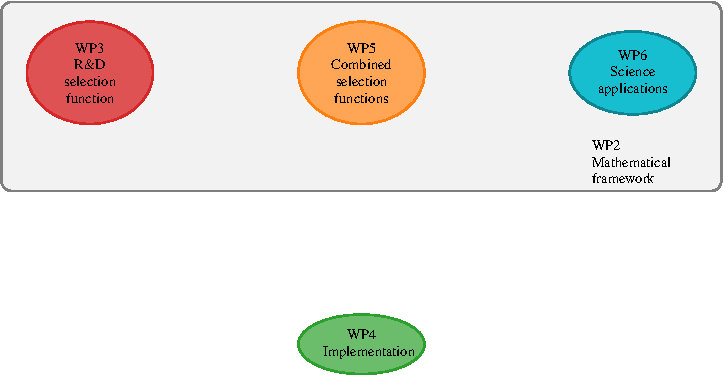
\includegraphics[width=\linewidth]{dependencies.pdf}
    \caption{The dependencies between the work packages in \acro.}
    \label{fig:dependencies}
\end{figure}

\section{Management structure, milestones and procedures}
\label{sec:management}

\subsection{Management}
\label{sec:mgtdetails}

The {\acro} consortium being relatively small the management structure can be kept simple in order to make the coordination of the efforts efficient. The management consists of three levels reflecting the structuring of the {\acro} work packages.
\begin{description}
    \item[Administrative management] This first level concerns the administrative management of {\acro}, including financial management and reporting to the European Commission. It is carried out by the {\acro} coordinator (A.~Brown) with the support of the Leiden Observatory institute management team.
    \item[Overall project management and coordination] This second level concerns the global scientific and technical control and coordination of the project, ensuring that the tasks are properly carried out and remain on schedule, and that the objectives of {\acro} are fulfilled. It is carried out by the \textbf{{\acro} executive board}, formed by the managers of the work packages: A.~Brown, R.~Drimmel, H.-W.~Rix, and V.~Belokurov. In order to keep communications within the consortium as efficient as possible the main contacts at NYU and MONA (D.~Hogg and A.~Casey) will have a standing invitation to attend the executive board meetings (see below).
    \item[Work package management] The third level of management concerns the main work packages. Each WP manager has the responsibility of supervising the execution of the core tasks assigned to their host institution, the work of the partners carrying out specific parts of the tasks attached to the work package, and report to the executive board accordingly.
    
    We do not further specify the management procedures for each work package beyond the items given in \secref{sec:procedures}, since the work in each of the work packages WP\ref{wp:selfundefinition} to WP\ref{wp:scienceappl} will be integrated in already existing and well established teams in each host institution.
\end{description}

This management structure together with the procedures described below is sufficient for a relatively small team spread over only six institutes working together closely in a scientific environment. Much of the coordination and supervision will take place through day-to-day contacts at the institutes involved and between institutes via e-mail and ad-hoc telecons. Similar structures were applied successfully to other EU-funded projects (FP7 GENIUS Collaborative project, FP7 GREAT Marie-Curie Initial Training Network) in which the coordinator was an active participant.

\subsection{Innovation management}
\label{sec:innovationmgmt}

The aim of {\acro} is to develop and deliver a new product (the Gaia selection function and tools to apply it) to the market of astronomy researchers. The wish for a selection function for the Gaia survey has been expressed on numerous occasions, meaning that this product will readily find a large user base. In order to uncover opportunities the astronomical community will be engaged during the lifetime of {\acro} through the availability of a prototype implementation of the Gaia selection function. The users thereof will be asked for feedback in the form of missing features or desired improvements. Community feedback wll also be obtained through presentation of {\acro} results at relevant scientific conferences.

\subsection{Procedures and reporting}
\label{sec:procedures}

We list here the procedures that will apply to the management of {\acro}:
\begin{itemize}
    \item The {\acro} coordinator will report to the European Commission following the rules applicable for research and innovation projects within the Horizon 2020 programme.
    \item {\acro} will hold at least three plenary meetings open to participation of all its members: the kick-off, mid-term, and closing meeting. The participation of the partner institute coordinators (or a representative) will be mandatory. Other plenary meetings may be held if needed.
    \item Specialized meetings or workshops will be organized on an `as-needed' basis by the WP managers.
    \item The executive board will hold teleconferences at least once a month to track the status of the tasks. The minutes of these teleconferences will be made available to the members of the consortium.
    \item The executive board shall ensure the coordination of the {\acro} work with the wider activities on the Gaia mission and its data releases, in particular ensuring the coordination with ESA and DPAC (see \secref{sec:dissemination-exploitation}). This can be done efficiently through membership of several {\acro} team members in DPAC.
\end{itemize}

\subsection{Consortium agreement}
\label{sec:cons_agreement}

The internal workings of {\acro} and the roles and responsibilities of the partners will be formalized through a consortium agreement which will be drawn up and agreed at the start of the programme. It will define the decision taking procedures in {\acro} and the mechanisms for conflict resolution, which will be channelled through the Executive Board, as well as the management of intellectual property rights as described in \secref{sec:openipr}.

\subsection{Recruitment strategy}
\label{sec:recruit}

The recruitment policy for {\acro} will conform to the principles of the European Charter for Researchers and the Code of Conduct for their recruitment. It will take place in a globally coordinated way during the six-month setup phase described in \secref{sec:wptiming}, placing an emphasis on individual excellence and capacity for team working, while taking care to ensure equal opportunity and gender balance.

%%%%%%%%%%%%
% MILESTONES
%%%%%%%%%%%%

\milestone[1]{Kick-off meeting}{Organized by {\acro} executive board}{WP\ref{wp:management}}
\milestone[4]{Hiring of researchers}{Partners notify {\acro} executive board}{WP\ref{wp:management}}
\milestone[12]{Document on mathematical formulation of selection function submitted to peer-reviewed journal}{Document approved by {\acro} executive board}{WP\ref{wp:selfundefinition}}
\milestone[18]{Document describing the preliminary Gaia selection function.}{Document approved by {\acro} executive board}{WP\ref{wp:selfungaia}}
\milestone[20]{Public prototype V1 of selection function implementation}{Software and data released and validated by user group}{P\ref{wp:selfunimplementation}}
\milestone[21]{Community workshop and mid-term meeting}{Organized by {\acro} executive board}{WP\ref{wp:management}}
\milestone[31]{Public prototype V2 of selection function implementation}{Software and data released and validated by user group}{WP\ref{wp:selfunimplementation}}
\milestone[32]{Community workshop}{Organized by {\acro} executive board}{WP\ref{wp:management}}
\milestone[36]{Papers and documentation describing the Gaia and combined selection functions ready to submit to peer-reviewed journals}{Verified by {\acro} executive board}{WP\ref{wp:selfungaia}, \ref{wp:selfunimplementation}, \ref{wp:selfuncombine}}
\milestone[41]{Closing meeting and community workshop}{Organized by {\acro} executive board}{WP\ref{wp:management}}
\milestone[42]{Publicly available selection function implementation, tools and data}{Software and data released and validated by user group}{WP\ref{wp:management}, \ref{wp:selfunimplementation}}

\makemilestoneslist

%%%%%%%
% RISKS
%%%%%%%
\criticalrisk{Late recruitment of researchers. Medium}{WP\ref{wp:selfungaia}--\ref{wp:scienceappl}}{Six month preparatory phase added in schedule to accommodate early advertizing of open positions. Use professional network of {\acro} participants. Executive board will track recruitment.}
\criticalrisk{Recruited researchers leaving early. Medium}{WP\ref{wp:selfungaia}--\ref{wp:scienceappl}}{Keep staff motivated, including through supporting career development. Coordinator and executive board will monitor personnel happiness.}
\criticalrisk{Unexpected complexity of tasks. High}{WP\ref{wp:selfungaia}--\ref{wp:scienceappl}}{Prioritize the {\acro} efforts and make timely decisions on dropping tasks deemed too complex.}
\criticalrisk{Lack of information from DPAC. Low}{WP\ref{wp:selfungaia}--\ref{wp:selfuncombine}}{{\acro} team members will be embedded in DPAC. Coordinator can identify alternative routes within DPAC to obtaining information.}
\criticalrisk{Coordination problems with ESA and DPAC leading to the selection function data products not being available through ESA archives. Low}{WP\ref{wp:selfunimplementation}}{Plan for alternative distribution channels. Coordinator to maintain close connections to ESA and DPAC.}
\criticalrisk{Delay of Gaia data releases. Can lead to difficulties in coordinating with DPAC/ESA (due to their prioritizing working on the releases). Medium}{WP\ref{wp:selfungaia}--\ref{wp:scienceappl}}{Coordinator to monitor the situation and agree mitigation measures with ESA/DPAC. We stress that even in the extremely unlikely case that no further Gaia data releases were to happen, the {\acro} effort will still have a major impact on the exploitation of the existing Gaia DR2 data.}

\makerisklist

\section{Consortium as a whole}
\label{sec:consortium}

The idea for this proposal grew out of discussions at several Gaia Sprints\footnote{\url{http://gaia.lol}} in which all of the {\acro} members participated, Hogg, Casey, Price-Whelan, and Rix being members of the organizing team of the Sprints. In particular at the Gaia Sprint that took place in Santa Barbara (USA) in March 2019, two sessions were dedicated solely to discussing the Gaia selection function. It was concluded that only a significant and dedicated effort, specifically funded, could realistically lead to the construction of the Gaia selection function and the corresponding tools and data needed to use it.

The consortium represents a combination of Gaia/DPAC experts (Brown, Drimmel, Fouesneau), experts that have given much thought to the principles of selections functions and worked on aspects of the Gaia selection function (Hogg, Rix, Drimmel, Price-Whelan, Casey, Fouesneau). All the participants have undertaken scientific analyses of the Gaia data that clearly highlight the need for a selection function. \memo{Look up relevant publications.}
\begin{itemize}
    \item The Gaia expertise in the consortium is contributed by long-standing DPAC members who are deeply involved in the data processing for the Gaia mission. They provide expert insight into the detailed ingredients of the Gaia selection function and, more importantly, have an extensive network of contacts with experts in DPAC who can provide more detailed information where needed. The presence of the Gaia experts is crucial to the guidance of the researchers to be funded through {\acro}. We note that the other participants have extensive experience as users of Gaia data and thus bring an important complementary perspective to {\acro}.
    \item The expertise on the mathematical formulation of the selection function and on selection functions in general is essential to the success of {\acro}. The expertise stems from the actual construction of selection functions and applying these to analyses of a number of large surveys \memo{(Example citations)}.
    \item The requirements on a selection function and how it is provided in its practical form must be guided by the experience gained through advanced scientific analyses of data such as from the Gaia mission. The experience from successes and failures in past analyses will be very important in setting the priorities for the research \& development in {\acro}.
\end{itemize}

The partners from Australia and the USA contribute deep knowledge of selection function issues based on their past scientific work. Their perspective as experienced users of the Gaia data will be essential to ensure that the developments in {\acro} stay focused on satisfying the needs of the astronomical community in general, and not just the needs of DPAC experts.

The participants in {\acro} have a long track record of effective collaboration as can be seen from the many joint publications. In addition good connections exist to experts who have already taken concrete steps to providing a Gaia selection function implementation, such as Boubert \& Everall\footnote{\url{https://github.com/DouglasBoubert/selectionfunctions}} (Oxford, Cambridge) and Rybizki\footnote{\url{https://github.com/jan-rybizki/gdr2_completeness}} (Heidelberg). Through the organization of Gaia Sprints and other workshops\footnote{For example the Gaia DR2 Exploration Lab \url{https://www.cosmos.esa.int/web/gaia-dr2-exploration}.} the participants have a proven track record of engaging the astronomical community, an important aspect of making sure that the tools and data delivered by {\acro} fulfil actual user needs.

The coordinator, A.~Brown, is also a member of the management committee of the COST action CA18104 `Revealing the Milky Way with Gaia'\footnote{\url{http://www.mw-gaia.org/}} and is co-I on the recently submitted proposal for a Marie Sk\l{}odowska-Curie Innovative Training Network also called `Revealing the Milky Way with Gaia'. We foresee participation in the conferences organized through the MW-Gaia COST action as part of the dissemination activities and if the ITN proposal is successful we would offer training in the use of the Gaia selection to the PhD students in that network. This could take place for example at one of the schools planned by the ITN, or through participation of the PhD students in our planned community workshops (deliverables \ref{dev:wp1midtterm}, \ref{dev:wp1community}, \ref{dev:wp1closing}).

\section{Resources to be committed}
\label{sec:resources}

\makesummaryofefforttable

\costsTravel{ULEI}{2500}{Explain}
\costsEquipment{ULEI}{3000}{Not needed probably}
\costsOther{ULEI}{60000}{TBD}

\makecoststable

%%% Local Variables:
%%% mode: latex
%%% TeX-master: "proposal-main"
%%% End:
